\documentclass[times, utf8, diplomski, english]{fer_eng}
\usepackage{pdfpages}
\usepackage{listings}
\usepackage{color}
\usepackage{natbib}
\usepackage{graphicx}
\setcitestyle{numbers}
\setcitestyle{square}
\lstset{
basicstyle=\ttfamily,
breaklines=true,
backgroundcolor=\color{lightgray}
}

\begin{document}

\thesisnumber{3028}

\title{Using Graph Neural Networks to Separate Haplotypes in Assembly Graphs}

\author{Filip Wolf}

\maketitle

% Ispis stranice s napomenom o umetanju izvornika rada. Uklonite naredbu \izvornik ako želite izbaciti tu stranicu.
\includepdf[pages=-]{"hr_0036510053_56.pdf"}

% Dodavanje zahvale ili prazne stranice. Ako ne želite dodati zahvalu, naredbu ostavite radi prazne stranice.
\zahvala{}

\tableofcontents

\chapter{Introduction}

Traditionally, the focus of \textit{de novo} genome assembly has always been on the reconstruction of an individual's genome from its numerous broken-up fragments obtained after sequencing \cite{de_novo2}. We will here, however, focus on a different application of \textit{de novo} genome assembly: haplotype separation. Every individual's genome is composed of both a mother's and a father's genome. Because we inherit both parent's chromosomes, the genetic material gets mixed between them, but some regions stay together in the form of genes. The term haplotype refers both to these inherited regions, as well as all of the genes of a parent on a chromosome \cite{haplotype}. In this thesis, we will use the term haplotype in the latter sense. By separating the two haplotypes from a genome, we can determine which parent contributed to what genes. This has a wide range of applications, from ancestry tests to finding hereditary diseases \cite{haplotype_usage}.         

We will try to do this using novel algorithms from the field of \textit{deep learning} (DL). Bioinformatics has long been dominated by algorithms that employ complex heuristics and expert knowledge to find solutions to the problems researchers face. This is however slowly changing. More and more research is being done using deep learning to solve problems in bioinformatics, foregoing the laborious process of feature engineering and extensive human intervention. First, DL was employed only for finding dense and abstract representations of genome features, but it later started to completely replace the previously mentioned algorithms. It has contributed tremendously to the field in recent years and shows no signs of stopping, the most notable achievement being the solution to the protein folding problem which previously wasn't solvable for 50 years \cite{alphafold}. Still, there remains a long way to go before DL becomes completely standard within the field. Thus, this Thesis is concerned with applying recent DL techniques in order to solve the problem of separating the two haplotypes in an existing genome. This could not only potentially improve performance and reduce the necessity for human experts, but also bring bioinformatics to a wider range of people \cite{dl_bioinformatics}.

\section{Bioinformatics}

Bioinformatics is an interdisciplinary field of research that has had a tremendous impact on humanity in the last few decades. Since the completion of the Human Genome Project \cite{HGP1} \cite{HGP2}, the cost of sequencing a human genome has fallen exponentially. We can now reliably sequence a human genome for less than a \$1000 \cite{genome_cost}, all thanks to recent advances in sequencing technology, as well as the accompanying algorithms. We will here briefly explain the general pipeline of genome sequencing, as well as the file formats used in the process.

\subsection{The Process of Sequencing and Assembly}
\label{The Process of Sequencing and Assembly}

In an ideal world, we would extract a human genome in the form of DNA from a cell, input it into a sequencer, and get a complete and accurate sequence of DNA as output which we could immediately use for further study. However, unfortunately this is not (yet) the case and it is hard to predict when this might become possible. Due to this, we have to make due with sequencers that can only output genomes in the form of thousands of fragmented reads, at maximum about 10 kilobases (kb) long, with shorter read sequencers sequencing reads at lengths of around 150 base pairs (bp). This process is called \textit{shotgun sequencing}. An average genome is much longer than that, e.g. the yeast genome is around 12 Mb long \cite{yeast} and the human genome is around 6.4 Gb long \cite{human}, so after sequencing, we need to assemble these short reads into longer ones before going deeper into analysis.

This process of finding longer reads is the first step in the process of \textit{assembly}. These longer reads are called \textit{contigs}. After this is done, we move on to looking for overlaps between the contigs which we use to create a graph in which each node represents a read, and each edge represents an overlap between reads. An overlap can be described as a match between two contigs' \textit{ends}, that is, the contig's prefix (start) and suffix (end). The length of this overlap can indicate a stronger similarity, and therefore stronger link between two contigs. Finally, we are tasked with finding the longest possible path on this graph to connect the individual contigs and form a complete genome.

%TODO: create image of de novo genome assembly

\subsection{File Formats}

As a specific subfield that combines computer science and genetics, bioinformatics uses multiple file formats that are unique to it. Mostly used for storing representations of genomic data, they offer us a simpler way to work with such data, as well as modify it. In the following sections, we will briefly describe these file formats, as well as state their usage in this project.

\subsubsection{FASTA \& FASTQ}

The most common file format encountered while working with genomic data is the FASTA format, designated by its .fasta or .fa file extension. It is a text-based format for storing nucleotide sequences and their information. Base pairs of amino acids are stored using letters (A - adenine, C - cytosine, G - guanine, T - thymine) in the form of a sequence. Every sequence starts with a description line, which is designated with a ">" symbol at the start of it. The description line can contain various information about the sequence, such as sequence name, sequence length, sequence statistics, etc. In our case, for the yeast genomic data, it specified the species and chromosome to which the sequences belonged to. After generating the reads (\ref{dataset}) for our data, the description contained data such as the read number, strand information, position on the chromosome, length and the chromosome to which it belonged to, as well as if its a mutated read or not. Sometimes, we may also encounter a FASTQ file. It is identical to a FASTA file, but with added sequence quality score information added after every sequence. In the following, we can see an example of a FASTA file filled with reads:

\begin{lstlisting}
>read=1,reverse,position=1004750-1015277,length=10527,NC_001139.9
AAGCTTGCAGATTTATTAACAGTTCAAACGAGTTTGGCTGATAATGCTCGTGCAGGTATTG
\end{lstlisting}

\subsubsection{CSV}

After generating various information about our dataset, we would store it in a CSV (comma separated values) file. That way, it could be easily read by some of the tools we used. A CSV file can be thought of as a table, where values in a row are separated with a comma sign. The file starts with a header with column names that are also separated with commas.

Another reason why we use the CSV file format is because of the Raven assembler outputting a CSV file with information about sequence overlaps. It is stored in the file in the following way. We start in a descending order of read name. A line with an even index number represents an original read, while a line with an odd index number line represents a \textit{virtual} read, i.e. a \textit{reverse complement} of the original read. A reverse complement represents the same sequence as the original, but in reverse order and with the base pairs replaced with their complements (A - T, C - G). The original and the reverse complement essentially represent the same genomic data, but on different strands of the DNA. An example of such a file is in the following:

\begin{lstlisting}
6549 [3274] LN:i:9216 RC:i:1,6412 [3206] LN:i:11360 RC:i:1,1,39678 8937 0 0.992832
6413 [3206] LN:i:11360 RC:i:1,6548 [3274] LN:i:9216 RC:i:1,1,39679 11081 0 0.992832
6647 [3323] LN:i:10656 RC:i:1,6638 [3319] LN:i:10224 RC:i:1,1,39680 10347 0 0.990291
6639 [3319] LN:i:10224 RC:i:1,6646 [3323] LN:i:10656 RC:i:1,1,39681 9915 0 0.990291
\end{lstlisting}

First, we have the index of the read. Then, in square brackets, we have the index of the original read (each virtual read forms a pair with an original read). Then, we have some read information, followed by the second read and its own information. Lastly, we have three fields that represent the overlap length, the weight of the overlap (here not used) and its score, measured in percentage of the overlap match respectively. Each line essentially represents an edge in our graph between two nodes. The first $n$ lines in the file, where $n$ is the number of reads, represent the overlap between the original and virtual file.

\subsubsection{GFA}

Another important file Raven outputs is a Graphical Fragment Assembly (GFA)\footnote{https://gfa-spec.github.io/GFA-spec/GFA1.html} file. It contains similar information to the CSV file, but with some notable additions, namely, instead of just specifying read overlaps, it also contains the whole sequences it uses in the assembly process. It also includes the original read names specified before assembly that contain mutation information. Each line in the file starts with an identifier, listed in the following table:

\begin{center}
	\begin{tabular}{ |c|c| }
		\hline
		\textbf{Type} & \textbf{Comment} \\
		\hline
		\# & Comment \\
		\hline
		H & Header \\
		\hline
		S & Segment \\
		\hline
		L & Link \\
		\hline
		C & Containment \\
		\hline
		P & Path \\
		\hline
		W & Walk \\
		\hline
	\end{tabular}
\end{center}

For our purposes, the file only contained lines starting with the letters S and L. S denotes a segment (sequence) used in the assembly, along with most of its information that was present before assembly (this is notable because it is missing in the CSV file). The lines starting with an L contain lines about sequence overlaps in a similar manner to the CSV file, with the addition of overlap length information and mutation info the later being crucial for specifying which edges connect what parent's haplotype. An example of lines starting with an L is in the following:

\begin{lstlisting}
L	read=4158,reverse,position=395590-406211,length=10621,NC_001139.9|mutated	+ read=4884,reverse,position=383506-395832,length=12326,NC_001139.9|mutated	+	101M
L	read=4832,forward,position=802633-815655,length=13022,NC_001139.9|mutated	-	read=4165,reverse,position=793088-803478,length=10390,NC_001139.9|mutated	+	733M
\end{lstlisting}

\subsubsection{Miscellaneous}

Aside from the mentioned file formats, we created numerous files of our own that either didn't have a suffix, or simply ended with a \textit{.txt} extension, for easier reading and writing. Those files were of an unspecified format and contained temporary information abut the graph, such as overlap lengths, parent affiliation, and similar.

\section{Thesis Task}

The task we are presented with here is slightly different compared to standard genome sequencing. Instead of just finding a path through the graph in order to assemble a complete genome, we are instead tasked with removing edges in the graph that connect contigs belonging to separate parents. By doing this, we are essentially separating the two haplotypes that constitute a genome. To give more insight into this, we will explain what graphs are and how we use them.

\subsection{Graphs}

Graphs are data structures that can be defined with a set of nodes (vertices) $V$ and a set of edges connecting them $E$. Formally, this can be written as:

\[ G = (V, E) \]
where:

\[ E \subseteq 	\{ (x, y)|(x, y) \in V^2 \mathrm{\ and\ } x \neq y \} \]
The above definition is an example of a directed graph, meaning that the edges only go in one direction, which is the type of graph we will work with. For instance, if edge $e$ is connecting nodes $v_1$ and $v_2$ in the direction $v_1 \rightarrow v_2$, then this means that node $v_1$ is connected to node $v_2$, but not the other way around. This is done because edge direction can encode both suffix - prefix and prefix - suffix overlaps, which is an useful information for us \cite{trudeau_2017}.

I this thesis, after sequencing and assembly (\ref{The Process of Sequencing and Assembly}), we obtain a list of reads connected to each other via overlaps. The reads can be thought of as nodes in a graph, while edges are the links between the nodes. By building such structures, we can more easily use existing graph theory insights to remove unnecessary edges and separate the two haplotypes.

\section{Deep Learning}

In this section, we will go over the basics of deep learning (\ref{subsec:basics}), the main tool used for the experiments in this thesis, followed with an overview of graph neural networks (\ref{subsec:graph neural networks}) and all its different variants we used.

\subsection{Basics}
\label{subsec:basics}

In the last decade, deep learning has grown from a niche research area to one of the largest fields withing computer science. It is now actively employed in virtually every human endeavor, from healthcare to entertainment \cite{dl_applications}. And it is still growing day by day on its mission to become the standard way of handling almost all data \cite{dl_growth}.

In deep learning, we use data processing structures called \textit{artificial neural networks} (ANNs) to extract useful information from our data and learn to predict an outcome, such as some feature of the data or a target class. ANNs do this by adjusting learnable \textit{weights} defined for every neuron in our network. Due to these weights, neural networks are much denser structures when compared to previous machine learning methods and can be referred to as \textit{universal function approximators} \cite{uni_approx} due to their ability to, with large enough networks, approximate any function. This gives them unprecedented performance on previously unsolvable tasks, but due to their abstract structure, makes them somewhat difficult to interpret. Some networks, like \textit{convolutional neural networks} \cite{CNN}, don't suffer from this problem as much and can produce some quite intuitive visualizations. On the other hand, some networks, like the ones we will use here, cannot be visually meaningfully interpreted.

To successfully explain how ANNs work, we need to introduce two concepts: a loss function and backpropagation. When use our deep learning model to learn from data, we pass it through our network and compare the output to a previously defined true value by using a \textit{loss function}. A loss function abstracts the error of our network prediction to a single number which is then used to calculate gradients in respect to our data. These gradients are then propagated back through the network using \textit{backpropagation}. In essence, the backpropagation algorithm tells every weight in our network how to change in order to better predict our data. If we imagine our data as a 2-dimensional function on a plane, a gradient is the information of how steeps the function is at any specified point. This steepness value tells the network weights how much they should change, while its sign specifies the direction of change. By correctly propagating these gradient values back through the network, which backpropagation does, we an successfully make our network learn from data \cite{Goodfellow-et-al-2016}.

\subsection{Graph Neural Networks}
\label{subsec:graph neural networks}

While standard ANNs are great at predicting simple data with no underlying structure (or at least one that isn't known), to successfully make our network learn from assembly graphs, we will need something more refined. Yes, it is true that we can simply represent our graph in the form of a 1-dimensional vector, but we then lose precious structural information about the contig overlaps. By using networks more tailor-made for data representation on graphs, we can take advantage of the graph's underlying structure. The networks in question are called \textit{Graph Neural Networks} (GNNs) \cite{GNN}. Most modern graph neural networks work on the principle of \textit{message passing} \cite{message_passing}. A node accumulates information from adjacent nodes and the edges connecting them and uses it to update its own weights. By repeating this process enough times, we can converge to a stable solution. This can be represented wit the following equation.

%napisati svojim rijecima

Let $x_v \in \mathbf{R}^{d_1}$ be the feature for node $v$, and $w \in \mathbf{R}^{d_2}$ be the feature for edge ($u$, $v$). The message passing paradigm defines the following node-wise and edge-wise computation at step $t+1$:

Edge-wise: $m_e^{(t+1)} = \phi (x_v^{(t)}, x_u^{(t)}, w_e^{(t)}), (u, v, e) \in \mathcal{E}$.

Node-wise: $x_v^{(t+1)} = \psi (x_v^{(t)}, \rho (\{m_e^{(t+1)}: (u, v, e) \in \mathcal{E}\}))$.

In the above equations, $\phi$ is a message function defined on each edge to generate a message by combining the edge feature with the features of its incident nodes; $\psi$ is an update function defined on each node to update the node feature by aggregating its incoming messages using the reduce function $\rho$.

The GNN can be though of as an extension of CNNs. A CNN takes an image's local neighborhood and extracts information from it. It does this using convolution \textit{filters}, which take a certain amount of pixels in a neighborhood and multiply them with weights. Now, the size of this filter is predefined and cannot be changed. For instance, it can have a size of 3 x 3 or 5 x 5. If we were to create such a filter for use on graphs, we would simply designate the central weight of the filter to be the node we are currently looking at, and the surrounding weights would be its neighboring nodes. As we can see, this would limit us to graphs where nodes had a constant number of neighbors, or graphs where we could look only at a limited number of neighbors. GNNs do not have this limitation. The $\psi$ function takes all nodes in a central node's neighborhood into account equally \cite{GRL} \cite{bronstein2021geometric}.

We used three different GNNs in this thesis, which we will describe in the following sections.

\subsubsection{Graph Covolutional Networks}

The first network we used was the simplest and oldest one, and it bases its computations on Graph Convolutional Networks (GCN) \cite{GCN}. It aggregates information from neighboring nodes and the edges connecting them and uses them to update the central node's information. It can be defined as follows:

\[ h_i^{(l+1)} = \sigma (b^{(l)} + \sum_{j \in \mathcal{N}(i)} \frac{e_{ji}}{c_{ji}} h_j^{(l)} W^{(l)} ) \]
Here, $\mathcal{N}(i)$ represents all the neighboring nodes of node $i$, $e_{ji}$ is the scalar weight of the edge connecting nodes $i$ and $j$, $c_{ji} = \sqrt{|\mathcal{N}(j)|} \sqrt{|\mathcal{N}(i)|}$, and $\sigma$ is an activation function. $b^{(l)}$, $h_j^{(l)}$ and $W^{(l)}$ are the networks bias at step $l$, features of node $j$ at step $l$ and weight of the network at step $l$ respectively. The aggregated information is used to update the features $h$ of node $i$ at step $(l+1)$. We can see that the calculations use are fairly straightforward, as they can be summed up by simply multiplying the network weight and node features and adding bias before passing it through an nonlinearity. A reader familiar with deep learning may notice that this is similar to an iteration of the backpropagation algorithm, but applied to the graph domain.

\subsubsection{Graph Attention Networks}
\label{Graph Attention Networks}

The second networks we used is more complex than a simple GCN, as it uses the \textit{attention mechanism} \cite{attention} to improve its performance. The Graph Attention Networks (GAT) \cite{GATv2} we used is an updated version of the original GAT \cite{GAT} called GATv2 and we did notice a slight increase in performance while using it. It can be defined as follows:

\[ h_i^{(l+1)} = \sum_{j \in \mathcal{N}(i)} \alpha_{ij}^{(l)} W_{right}^{(l)} h_j^{(l)} \]
where:
\[ \alpha_{ij}^{(l)} = \mathrm{softmax}_i (e_{ij}^{(l)}) \]
\[ e_{ij}^{(l)} = \vec{a}^{T^{(l)}} \mathrm{LeakyReLU} (W_{left}^{(l)} h_i + W_{right}^{(l)} h_j) \]
Here, $W_{right}$ is one of the two network weight matrices, $h$ is a node feature matrix, $\alpha$ is an attention weight and $\vec{a}$ is the attention weight vector. We can see that the basic equation is similar to the GCN, but with an added attention weight. This weight is the main reason why the network performs better compared to the regular GCN. The attention mechanism works by selecting data instances during training, such as nodes, that it considers more important than other data and thereby giving it more weight. This way, it increases model capacity and performance, while at the same time not directly increasing the network size. It is also worth mentioning that we can specify a number of so-called attention heads. Attention heads are simply multiple attention mechanisms at work at the same time. The final attention score is calculated by concatenating or averaging these different attention values. This is done to improve training stability and ultimately performance.

This network differs from the original GAT only in the way $e_{ij}^{(l)}$ is calculated. Instead of using a single weight matrix $W$ that is concatenated to the features $h$, we use two separate matrices in the form of $W_{right}$ and $W_{left}$, giving the network more parameters and learning power.

\subsubsection{Edge Graph Attention Network}

The last network we used, and by far the most effective one, is the graph attention layer that handles edge features (EGAT) \cite{EGAT}. The main equation is the same as in GAT (\ref{Graph Attention Networks}). The difference lies in how the attention scores $e_{ij}$ are calculated. Instead of the usual way, the are obtained like this:

\[ e_{ij} = \vec{a} f_{ij}^{'} \]
\[ f_{ij}^{'} = \mathrm{LeakyReLU} (A[h_i||f_{ij}||h_j]) \]
Here, $f_{ij}$ represents edge features, $A$ is a weight matrix and $\vec{a}$ is a weight vector. This network greatly improves performance due to the fact that it better utilizes edge features. Instead of just using them as weights to scale edge importance, it handles them in the same manner of importance as the node features. This way, the network can find meaning in the edge weights much better compared to a regular GAT network.

\subsection{Other Functions}

In this section, we will explain all the functions we use in our networks that aren't directly responsible for training, such as regularization functions and nonlinearities.

\subsubsection{Nonlinearities}
\label{subsubsec: nonlinearities}

%todo: add sigmoid description

We use three nonlinearities in our work, all of them quite similar to each other. The most basic one is the \textbf{ReLU} (rectified linear unit) \cite{relu}.	It can be simply described with the following equation:

\[ \mathrm{ReLU}(z) = \max (0, z) \]
In other words, it lets through everything that is positive in a linear fashion, and sets everything else to zero. This is one of the most widely used nonlinearities. It has the same benefits as a sigmoid function or a tanh function, but is less computationally expensive.

A variant of the ReLU is the \textbf{LeakyReLU} \cite{leakyrelu}. It only differs from ReLU in that it allows for a small non zero constant gradient $\alpha$ below zero. It tries to fix the limitation of ReLU where some neurons never express their values due to them being negative.

Finally, we have the \textbf{ELU} (exponential linear unit) \cite{elu}. It can be described with the following equation:

\[ \mathrm{ELU}(z) = \begin{cases} 
z & z > 0 \\
\alpha \cdot (e^z - 1) & z \leq 0
\end{cases} \]
For values greater than 0, it emits a constant output. But for any other value, it slowly smooths out bellow zero where it tends to the value $- \alpha$. Just like LeakyReLU, it also tries to negate some weaknesses of ReLU and can be used as a strong alternative to it.

\subsubsection{Regularization Functions}
\label{subsubsec:regularization functions}

We primarily used three different regularization functions throughout our networks. In general, these functions help stabilize and speed up network training, as well as often improve performance slightly.

Before imputing our data into the model, we \textbf{normalize} it. If this isn't done automatically in the network, we do it with built-in functions, which involves simply dividing an edge weight with all other edge weights connected to the same nodes.

More interesting that normalization is \textbf{dropout} \cite{dropout} \cite{dropout2}. Dropout is one of the most popular regularization techniques and often greatly improves network performance. It works by randomly omitting entire neurons from the network along with their connection. By doing this, neurons get more specialized in detecting different features in the data and don't co-adapt as much. In practice, these neurons aren't actually dropped, but their weights are simply reduced by multiplying them with small constants, thereby lessening their importance during training and subsequent prediction.

Lastly, we employed \textbf{batch normalization} \cite{bn}. During training, it normalizes the outputs of neurons so that the next layers can always expect the same kinds of values as input, thereby stabilizing and greatly improving training times. It also allows for a much wider range o learning rate values to be used without making the model diverge. As a side effect, by making the layer activations less dependent on the current batch, it adds some noise to training, and thereby acts as a regularizer to the network.

\chapter{Dataset}
\label{ch:dataset}

In this chapter, we will go over the dataset we used for our models. First, we will give an introduction to the dataset we chose to use and why we did so (\ref{sec:introduction}), and then explain how we generated our own dataset for use in our models (\ref{sec:dataset creation}).

\section{Introduction}
\label{sec:introduction}

When it comes to deep learning, data can often take a central role in determining the final outcome of the project. Although carefully crafting a predictive model is important, data quality can have a large impact on the model's performance. In this thesis, in order to train our model, we artificially created a dataset based on the brewer's yeast (\textit{Saccharomyces cerevisiae}) genome. For most experimentation purposes, this dataset was only created using the first chromosome of the genome, as using the entire genome required the creation of a much larger dataset that would have significantly slowed down the training and testing process of different models. This larger dataset would have been necessary due to the fact that using the same number of reads for a larger number of chromosomes than just one would essentially dilute our available information for each chromosome, making our models difficult to train. This can be mitigated by the fact that different chromosomes are somewhat similar, as we will see in further experiments. Nevertheless, using only one chromosome proved effective enough for testing out different models, as we will see later in the results section.

\section{Dataset Creation}
\label{sec:dataset creation}

There ar a lot of readily available datasets for experimenting on graphs and genomic data, but for our intents and purposes, we required a custom dataset created from our own data. We will explain in detail how we created this dataset and how we used it in our experiments.

\subsection{Simulating \& Mutating the Reads}

To generate the dataset, we used a multi-step process. The yeast genome was stored in a simple FASTA file with the chromosomes written down in order. In the first step, we would simply extract the first chromosome from the FASTA file. In the next step, in order to simulate a fragmented chromosome like if it was obtained in the process of sequencing, we needed to generate artificial reads from the chromosome. This was done using the \texttt{seqrequester}\footnote{https://github.com/marbl/seqrequester} package and its \texttt{generate} option for generating reads. By setting the \texttt{-nreads} flag to the desired number, we could specify the number of reads the program would generate, and using the \texttt{-distribution} flag, we could choose the desired distribution for the reads (in our case \texttt{pacbio-hifi}). After this was done, we ended up with a file filled with simulated reads. We used a small C++ program\footnote{Courtesy of R. Vaser} to mutate these reads into new ones of the same length with a mutation frequency of 0.01, meaning that every 100 base pairs, a base pair would get mutated into its complement base pair. Now, if the original simulated reads represented the mother's reads, these mutated ones could be thought of as the father's reads. Lastly, we combined them into a single file by simply concatenating them, and we were now ready for the final sequencing process where we would obtain contigs and their overlaps which we could use for training our model.

\begin{figure}[h]
	\centering
	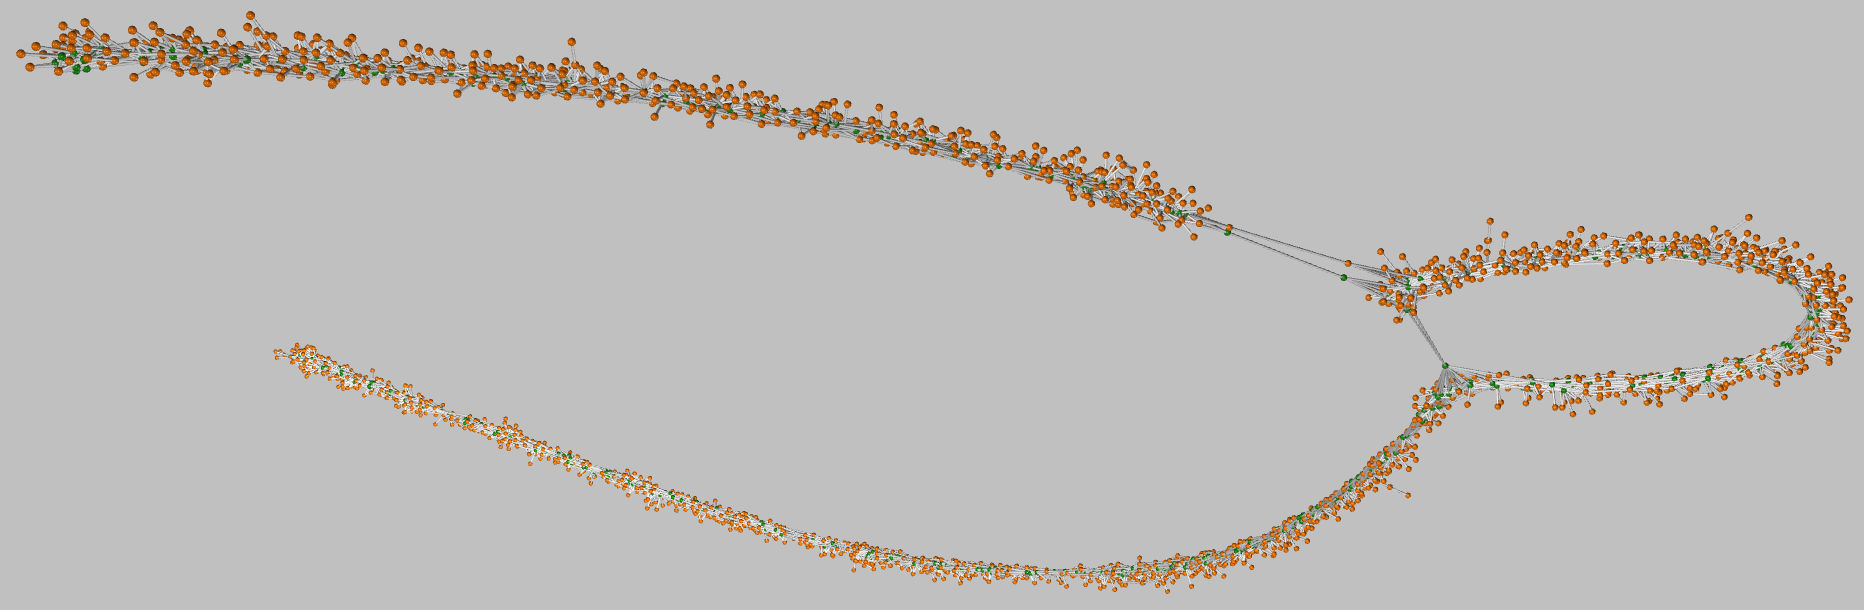
\includegraphics[width=\textwidth]{images/graph_example.png}
	\caption[Graph]{Example of a graph obtained after sequencing and assembly. Orange nodes represent mutated reads, while green nodes represent the original reads. This graph was obtained using the Graphia\footnotemark{} graphing tool.}
	\label{fig:graph}
\end{figure}
\footnotetext{https://graphia.app/}

\subsection{Assembling the Graph}

We found that generating 5000 - 10 000 reads gave satisfactory results in combination with the Raven assembler \cite{Vaser}. This is due to the fact that Raven's \texttt{filter} option reduces the number of edges in the graph if a smaller value for the option is specified. While setting the option to 0.99, and using the previously mentioned number of reads, Raven will generate an appropriate number of nodes and edges for training. Setting it to anything lower would create datasets too small for training. Unfortunately, this very low filter value also meant that the overlaps between our contigs were also a minimum of 99\%, making them less of a candidate for usage as edge features.

After Raven is done with the assembly process, it outputs two files: a GFA file and CSV file. They both contain information about the contigs and their overlaps suitable in a format for generating a graph. They also contained different information in each, so to fully utilize all the graph information we have available, we needed to use both files. From the GFA file, we extract information about which contig belongs to the mutated reads and which one to the original simulated ones, as well as contig overlap length information. We extract them to a separate file for easier analyzing. An example of a graph obtained after assembly can be seen in \ref{fig:graph}. Now, as we previously mentioned, our task is to separate the contigs into the father's and the mother's genome. In other words, if we are presented with a graph where nodes represent contigs and edges their overlaps, we need to remove edges between contigs that don't belong to the same parent. So for each edge, we specify if it's "correct" (i.e. it connects two contigs belonging to the same parent) or "incorrect" (it connect two contigs belonging to different parents). We now have a dataset where each edge has a label, as well as a feature in the form of overlap length. We can now use this as input to our model to generate a dataset fit for training.

\chapter{Implementation}

In this chapter, we will go over all the different software components we used for our experiments. First, we will go over the software we used for our deep learning models, as well as all the tools we used to help us (\ref{sec:technology stack}). After that, we will explain the structure of our model and how all the different components come together (\ref{sec:code structure}).

\section{Technology Stack}
\label{sec:technology stack}

The main programming language used for this thesis was Python\footnote{https://www.python.org/}, specifically, Python version 3.9. Aside from this, we also used Bash\footnote{https://www.gnu.org/software/bash/} in order to build some scripts to speed up repetitive tasks. Most of the core functionalities of this project were implemented using two Python libraries: PyTorch and DGL. PyTorch\footnote{https://pytorch.org/} probably needs no introduction. It is currently one of the most popular deep learning library used by millions due to its simplicity and versatility \cite{popular_ml}. It is free and open source and maintained by Facebook's AI Research lab. In this project, it was mostly used for its \textit{tensor} data structure, its implementation of nonlinearities such as the ReLU and ELU, and loss functions such as cross entropy loss and others. It is also used as the underlying architecture for the deep learning layers we used, which will be described in the next paragraph.

The Deep Graph Library\footnote{https://www.dgl.ai/} (DGL) \cite{DGL} is an free and open source deep learning library primarily aimed at the graph neural networks domain. It is maintained by a diverse team of contributors, most of the stemming from the Amazon Web Services team. In this project, it proved itself as a crucial addition to the list of used tools due to its numerous graph oriented functions. We used it mainly for the following features. Firstly, it allowed us to effortlessly and efficiently create graphs from our yeast dataset that were then used for training our models. Secondly, its numerous implemented GNN layers were easy to set up and test out, allowing us to more quickly find the best model for our data. Lastly, due to it being built on the previously mentioned PyTorch library, it had seamless integration with it and could use many of PyTorch's built in functions to help us in training.

Aside from this, we also used a few other libraries to help us in some tasks. We will here shortly list them and describe them.

\begin{itemize}
	\item NumPy\footnote{https://numpy.org/} - a popular Python library focused on efficient and easy mathematical calculations. We mostly used it for its implementation of large arrays

	\item Pandas\footnote{https://pandas.pydata.org/} - a Python data science library with numerous data oriented features. We used it for its CSV saving and loading capabilities

	\item Scikit-learn\footnote{https://scikit-learn.org/stable/} - the most popular machine learning library for Python. We used its easy to use performance metrics, such as F1 score and accuracy

	\item TensorBoard\footnote{https://www.tensorflow.org/tensorboard} - a Python library used for easy visualization of the training process and its metrics
\end{itemize}

\section{Code Structure}
\label{sec:code structure}

The project contained three main files as well as some helper scripts. In the following sections, we will describe these.

\subsection{DGLDataset}

The first thing to do was generate a dataset from the data obtained after sequencing. For this, we used DGLs \texttt{dgl.data.DGLDataset} class, which we inherit. It has multiple purposes, after generating a dataset we can save it and load it by calling the \texttt{save} and \texttt{load} functions. We can also check if there already is a previously saved dataset using the \texttt{has\_cache} function. We can also get an instance of the dataset by calling the \texttt{\_\_getitem\_\_} function, as well as its length using the \texttt{\_\_len\_\_} function. But by far its most important purpose is generating the dataset we will use for training. We do this by loading the previously generated node and edge features and using them to generate a graph. We also encode label information, edge features, and node features. Node features are generated by taking the in and out degrees of every node.

\subsection{Models}

The models we used for training are defined by inheriting the \texttt{torch.nn.Module} class. In each model, we define the layers of the network, as well as the \texttt{forward} function for the gradients calculation. An example of the EGAT model definition code is in the following:

\begin{lstlisting}
class EGATModel(nn.Module):
def __init__(self, node_features, edge_features, lin_dim, hidden_dim, out_dim, n_classes, num_heads):
super(EGATModel, self).__init__()
self.lin_n = nn.Linear(node_features, lin_dim)
self.egat1 = EGATConv(lin_dim, edge_features, hidden_dim, hidden_dim, num_heads=num_heads)
self.egat2 = EGATConv(hidden_dim * num_heads, hidden_dim * num_heads, out_dim, out_dim, num_heads=1)
self.egat3 = EGATConv(out_dim, out_dim, int(out_dim / 2), int(out_dim / 2), num_heads=1)
self.egat4 = EGATConv(int(out_dim / 2), int(out_dim / 2), int(out_dim / 4), int(out_dim / 4), num_heads=1)
self.classify = MLPPredictorEGAT(int(out_dim / 4), n_classes)
self.dp = nn.Dropout(p=0.5)
\end{lstlisting}

We define the network in the following way. First, we initalize a linear layer that transforms the node features (number of in and out node degrees) into a higher dimension of size \texttt{node\_features}. Then, we define four EGAT layers. The first layer is of the largest width \texttt{hidden\_dim} (both for node and edge features), and subsequent layers divide this size by two in each step. Only the first layer used a \texttt{num\_heads} number of attention heads, the rest used only one. This is done to improve training times, as this network proved much slower than the other ones we used. After all the EGAT layers are done with their computations, we pass everything through a classification layer. This layer works by taking the new calculated node and edge features and concatenating them before passing them into a fully connected classification layer. The network then finally outputs a list of class probabilities for every edge in the graph.

You may have noticed that in some layers, we multiply the input dimension for the EGAT layer with \texttt{num\_heads}. This is done so that the number of attention heads is accounted for correctly while passing the results to the next network. The different layer outputs are \textit{flattened}, i.e. concatenated into a smaller dimensional vector before being passed to the next layer. Aside from this, we also employ the \textit{dropout} \cite{dropout} mechanism to reduce overfitting.

\subsection{Main}

All of the previously described functions are connected in the \texttt{main} function. First, we define the function for logging parameters such as loss and accuracy for visualization using TensorBoard. Then, we define the dataset by calling the \texttt{DGLDataset} module and, if it previously hasn't been generated, create the dataset. We then define the model we will use for training with all its parameters and layer sizes. We define the optimizer, and finally, start the training process.

\begin{figure}[h]
	\centering
	\includegraphics[width=\textwidth]{images/model.png}
	\caption[Model]{Graphical representation of the model architecture with EGAT layers. Different layers are represented with different colors and the main model is described within the gray box.}
	\label{fig:model}
\end{figure}

\section{Model description}

In Figure \ref{fig:model}, we can see the general structure of one of our models, specifically, the model using the EGAT layers. We will explain this model in detail as it is the most complicated one we used and it generalizes well to all other models we used.

In the first step, we take node features, node in and out degrees, as input to a linear layer. The dimension of each of these feature vectors is $n$, where $n$ is the number of nodes in the current graph. The purpose of this linear layer is to increase the size of the features from two to a larger number $m_1$ (usually 64 or 128), thereby extracting useful information from them and successfully representing it with a suitable dimension.

We then have $n \times m_1$ matrix, which we use as input to the first EGAT layer along with the node features we use (edge overlap lengths) and the graph structure. The EGAT layer uses these to perform its operations and outputs two vectors of size $n \times m_2 \times a$ and $e \times m_2 \times a$, where $m_2$ is the output size of the first EGAT layer (usually larger than $m_1$), $a$ is the number of attention heads (usually three) and $e$ is the number of edges. The two vectors represent the learned features of the nodes and edges respectively. They are then passed through ELU activation function (Section \ref{subsubsec: nonlinearities}) which acts as a nonlinearity, followed with the dropout mechanism (Section \ref{subsubsec:regularization functions}). This is then finally passed through batch normalization (Section \ref{subsubsec:regularization functions}).

This set of operations represents one step of the network, which we perform four times. In each step, we reduce the $m_2$ dimension two times in each step and use only one attention head. After the final layer is done, we pass everything through a classification layer. This layer works by taking the last set of calculated node and edge features and concatenates them in a node feature, edge feature, node feature order. These are then used as input to a fully connected layer which finally outputs logits. To use them in a loss function, we pass them through a sigmoid function to get class probabilities.

%TODO: create diagram of how everything connects

\chapter{Results}

In this chapter, we will present the results obtained in the experiments we performed for this thesis. First, we will go over the experiments on only one chromosome (\ref{sec:experiments on one chromosome}), and then over the experiments on the whole genome.

\section{Performance Metrics}

Here, we will briefly explain all the different metrics for evaluating model performance during training that we used. These include accuracy, F1 score and model loss.

\subsection{Accuracy}

Accuracy is a simple and reliable metric foe assessing model performance that is quite popular and widespread due to its interpretability and it being easy to understand. It can be described as the number of correctly classified examples divided by the total number of examples in the dataset. With that said, it does have limits to its use. For instance, in the case when the dataset is severely imbalanced, i.e. there are many more examples of one class, e.g. \textit{true} compared to the other, e.g. \textit{false}, it will always display a high performance figure by simply always guessing \textit{true}. Fortunately, this is not the case for our dataset, as we have a fairly similar number of correct and incorrect examples. We can also define it with the following equation:

\[ \mathrm{Accuracy} = \frac{\mathrm{TP} + \mathrm{TN}}{\mathrm{TP} + \mathrm{TN} + \mathrm{FP} + \mathrm{FN}} \]

Accuracy is the number of \textit{true positive} and \textit{true negative} examples divided by all examples. In other words, it is the sum of everything our model classified correctly divided by both everything our model did and didn't classify correctly.

\subsection{F1 score}

F1 score is slightly more complex than the previously described accuracy score. It belongs to a family of scores known as \textit{F-scores}, which can be described with the following equation:

\[ \mathrm{F} = (1 + \beta^2) \cdot \frac{\mathrm{precision} \cdot \mathrm{recall}}{(\beta^2 \cdot \mathrm{precision}) + \mathrm{recall}} \] where \[ \mathrm{precision} = \frac{\mathrm{TP}}{\mathrm{TP} + \mathrm{FP}} \] \[ \mathrm{recall} = \frac{\mathrm{TP}}{\mathrm{TP} + \mathrm{FN}} \]
Precision measures how many of the examples we classified as postive are truly possitive, while recall measures how many of the positive examples we actually classified as positive.

F1 score is a version of the F-score where the $\beta$ parameter is set to 1, which in turn simplifies the equation to:

\[ \mathrm{F_1} = 2 \frac{\mathrm{precision} \cdot \mathrm{recall}}{\mathrm{precision} + \mathrm{recall}} \]
It can be described as the harmonic mean between the precision and recall metrics and is often used as a more data agnostic version of those metrics.

\subsection{Loss Function}

As our model falls into the classification category, for the loss function, we used \textit{cross entropy loss}, also know as \textit{logistic loss}. In works by taking the \textit{logits} our model outputs and comparing them against the true labels. Logits are vectors of size $n$, where $n$ is the number of classes we're predicting for every data entry. For instance, if we have 3 examples in our dataset that we need to classify and 7 classes, the size of our matrix would be $7 \times 3$. This matrix is compared to the \textit{one-hot} encoded classes of the data. One-hot encoded vectors are also of size $n$, but with only their true class for the example set to 1, and everything else to 0. They are compared with the following equation:

\[ L = - \sum_{i = 1}^n t_i \log (p_i) \]
where $t_i$ is either a 1 or a 0 (truth label) for class $i$, and $p_i$ is the probability for class $i$. If we are only using two classes (which we indeed are), we can simplify this to \textit{binary cross entropy loss} represented with the following equation:

\[ L = - [t \log (p) + (1 - t) \log (1 - p)] \]
A smaller value is better, so by minimizing this loss, we can train our model. Due to its logarithmic nature, it heavily penalizes values straying from 0, which is the ideal value of the function \cite{CEL}.

It is also worth noting that the model doesn't take logits as input directly, but class probabilities instead. Therefore, before passing them to the function, we have to pass the logits through a \textit{softmax} function to normalize them into a range between 0 and 1 s that they can be interpreted as probabilities. The softmax function, or \textit{sigmoid} function if only two classes are present, can be described with the following equation:

\[ \sigma(x) = \frac{\exp (x_i)}{\sum_j \exp (x_j)} \]
In other words, we simply divide the exponent of our logit value by all logit exponents.

\section{Experiments on One Chromosome}
\label{sec:experiments on one chromosome}

The results of the experiments we performed on the dataset are presented through three graphs: accuracy, F1 score and loss. We will only display validation graphs, as training graphs are often an unreliable indicator of performance and they almost certainly overfit. In addition, we will only display a few different experiments we performed for clarity, even there were many more. Lastly, we only display the first 200 epochs of training, as all of the models reached their peak performance up to this point.

\subsection{Accuracy \& F1 Score}

\begin{figure}[h]
	\centering
	\includegraphics[width=\textwidth]{images/accuracy_val.png}
	\includegraphics[width=\textwidth]{images/f1_val.png}
	\caption[Accuracy and f1 graph]{Two graphs representing the model training performance on the validation part of the dataset. Above, we have the accuracy graph and below it, we can see an F1 score graph. Epochs are displayed on the $x$ axis, while on the $y$ axis, we have the respective performance metric of either accuracy or F1 score. The graphs were obtained using TensorBoard.}
	\label{fig:accuracy and f1 graph}
\end{figure}

The first two graphs we are going to look at are an accuracy graph and an F1 score graph (\ref{fig:accuracy and f1 graph} top, \ref{fig:accuracy and f1 graph} bottom). We are going to analyze both of them at the same time due to their similarity. There are four model results displayed here. In red, a GATv2 model with dropout set to 0.5 and edge overlaps used as edge weights in the GCN layers is displayed. In blue, we have the same model, but without using edge overlaps. Their performance is nearly similar, proving that this way of using edge overlaps is rather inefficient. In orange, we use GCN model with dropout set to 0.2 and edge overlaps used. We can see that it is of a very similar performance, meaning that the GAT layers extract little additional information from the model.

The standout model here is the pink model. It has greatly outperformed the rest of the models, with an accuracy of 87.9\%. This is because here we used an EGAT model, which uses edge features much more effectively by incorporating them into the attention mechanism. However, we have to note that we had to use a much smaller model here due to slow training times. Nevertheless, it proved effective for the task at hand.

\chapter{Conclusion}


\bibliography{literatura}
\bibliographystyle{abbrv}

\clearpage

\title{Using Graph Neural Networks to Separate Haplotypes in Assembly Graphs}
\begin{abstract}

\keywords{}
\end{abstract}

\hrtitle{}
\begin{sazetak}

\kljucnerijeci{}
\end{sazetak}

\end{document}